\documentclass[a4paper]{article}
\usepackage{geometry}
\usepackage{graphicx}
\usepackage{natbib}
\usepackage{amsmath}
\usepackage{amssymb}
\usepackage{amsthm}
\usepackage{paralist}
\usepackage{epstopdf}
\usepackage{tabularx}
\usepackage{longtable}
\usepackage{multirow}
\usepackage{multicol}
\usepackage[hidelinks]{hyperref}
\usepackage{fancyvrb}
\usepackage{algorithm}
\usepackage{algorithmic}
\usepackage{float}
\usepackage{paralist}
\usepackage[svgname]{xcolor}
\usepackage{enumerate}
\usepackage{array}
\usepackage{times}
\usepackage{url}
\usepackage{fancyhdr}
\usepackage{comment}
\usepackage{environ}
\usepackage{times}
\usepackage{textcomp}
\usepackage{caption}
\usepackage{color}
\usepackage{xcolor}

\urlstyle{rm}

\setlength\parindent{0pt} % Removes all indentation from paragraphs
\theoremstyle{definition}
\newtheorem{definition}{Definition}[]
\newtheorem{conjecture}{Conjecture}[]
\newtheorem{example}{Example}[]
\newtheorem{theorem}{Theorem}[]
\newtheorem{lemma}{Lemma}
\newtheorem{proposition}{Proposition}
\newtheorem{corollary}{Corollary}

\floatname{algorithm}{Procedure}
\renewcommand{\algorithmicrequire}{\textbf{Input:}}
\renewcommand{\algorithmicensure}{\textbf{Output:}}
\newcommand{\abs}[1]{\lvert#1\rvert}
\newcommand{\norm}[1]{\lVert#1\rVert}
\newcommand{\RR}{\mathbb{R}}
\newcommand{\CC}{\mathbb{C}}
\newcommand{\Nat}{\mathbb{N}}
\newcommand{\br}[1]{\{#1\}}
\DeclareMathOperator*{\argmin}{arg\,min}
\DeclareMathOperator*{\argmax}{arg\,max}
\renewcommand{\qedsymbol}{$\blacksquare$}

\definecolor{dkgreen}{rgb}{0,0.6,0}
\definecolor{gray}{rgb}{0.5,0.5,0.5}
\definecolor{mauve}{rgb}{0.58,0,0.82}

\newcommand{\Var}{\mathrm{Var}}
\newcommand{\Cov}{\mathrm{Cov}}

\newcommand{\vc}[1]{\boldsymbol{#1}}
\newcommand{\xv}{\vc{x}}
\newcommand{\Sigmav}{\vc{\Sigma}}
\newcommand{\alphav}{\vc{\alpha}}
\newcommand{\muv}{\vc{\mu}}

\newcommand{\red}[1]{\textcolor{red}{#1}}

\def\x{\mathbf x}
\def\y{\mathbf y}
\def\w{\mathbf w}
\def\v{\mathbf v}
\def\E{\mathbb E}
\def\V{\mathbb V}

% TO SHOW SOLUTIONS, include following (else comment out):
\newenvironment{soln}{
    \leavevmode\color{blue}\ignorespaces
}{}


\hypersetup{
%    colorlinks,
    linkcolor={red!50!black},
    citecolor={blue!50!black},
    urlcolor={blue!80!black}
}

\geometry{
  top=1in,            % <-- you want to adjust this
  inner=1in,
  outer=1in,
  bottom=1in,
  headheight=3em,       % <-- and this
  headsep=2em,          % <-- and this
  footskip=3em,
}


\pagestyle{fancyplain}
\lhead{\fancyplain{}{Homework 2}}
\rhead{\fancyplain{}{CS 760 Machine Learning}}
\cfoot{\thepage}

\title{\textsc{Homework 2}} % Titleß

\author{
RYAN YEE \\
9074025223\\
} 

\date{}

\begin{document}

\maketitle 


\textbf{Instructions:} 
Use this latex file as a template to develop your homework. Submit your homework on time as a single pdf file to Canvas. Please wrap your code and upload to a public GitHub repo, then attach the link below the instructions so that we can access it. You can choose any programming language (i.e. python, R, or MATLAB), as long as you implement the algorithm from scratch (e.g. do not use sklearn on questions 1 to 7 in section 2). Please check Piazza for updates about the homework.\\

Code used for this assignment can be found at \url{https://github.com/ryanyee3/CS760_Machine_Learning/tree/master/homework2}.

\section{A Simplified Decision Tree}
You are to implement a decision-tree learner for classification.
To simplify your work, this will not be a general purpose decision tree.  Instead, your program can assume that
\begin{itemize}
\item each item has two continuous features $\x \in \RR^2$
\item the class label is binary and encoded as $y \in \{0,1\}$
\item data files are in plaintext with one labeled item per line, separated by whitespace:
$$x_{11} \quad x_{12} \quad y_1$$
$$...$$
$$x_{n1} \quad x_{n2} \quad y_n$$
\end{itemize}

Your program should implement a decision tree learner according to the following guidelines:
\begin{itemize}
\item Candidate splits $(j,c)$ for numeric features should use a threshold $c$ in feature dimension $j$ in the form of $x_{\cdot j}\ge c$.
\item $c$ should be on values of that dimension present in the training data; i.e. the threshold is on training points, not in between training points. You may enumerate all features, and for each feature, use all possible values for that dimension.
\item You may skip those candidate splits with zero split information (i.e. the entropy of the split), and continue the enumeration.
\item The left branch of such a split is the ``then'' branch, and the right branch is ``else''.
\item Splits should be chosen using information gain ratio. If there is a tie you may break it arbitrarily.
\item The stopping criteria (for making a node into a leaf) are that 
	\begin{itemize}
	\item the node is empty, or
	\item all splits have zero gain ratio (if the entropy of the split is non-zero), or
	\item the entropy of any candidates split is zero
	\end{itemize}
\item To simplify, whenever there is no majority class in a leaf, let it predict $y=1$.
\end{itemize}

\section{Questions}
\begin{enumerate}
\item (Our algorithm stops at pure labels) [10 pts] If a node is not empty but contains training items with the same label, why is it guaranteed to become a leaf?  Explain. You may assume that the feature values of these items are not all the same. \\

\begin{soln}
  If a node is not empty but contains items with only labels, it is guaranteed to be a leaf because the information gain from any split will be zero.
  Indeed, suppose all the labels in the node are 1.
  Then for this node, $H(Y \vert X) = P(X = 1)H(Y \vert X=1) + P(X = 0)H(Y \vert X=0) = H(Y \vert X=1) = H(Y)$.
  Thus, $H(Y) - H(Y \vert X) = 0$ which is a stopping condition.
\end{soln}

\item (Our algorithm is greedy)  [10 pts] Handcraft a small training set where both classes are present but the algorithm refuses to split; instead it makes the root a leaf and stop;
Importantly, if we were to manually force a split, the algorithm will happily continue splitting the data set further and produce a deeper tree with zero training error.
You should (1) plot your training set, (2) explain why.  Hint: you don't need more than a handful of items. \\

\begin{soln}
  \begin{figure}[h!]
    \centering
    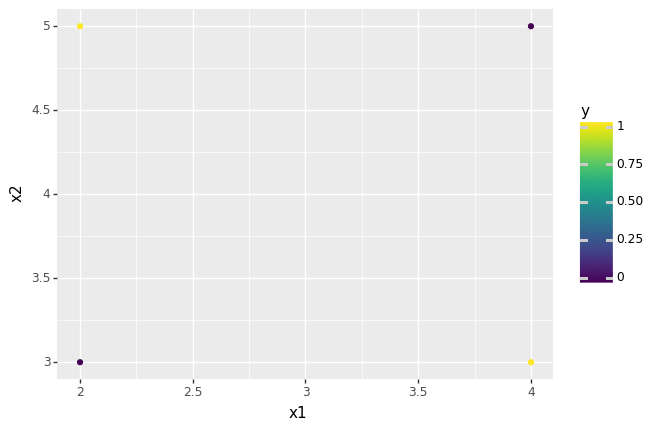
\includegraphics[width=0.8\textwidth]{../plots/q2_plot.png}
    \caption{Plot of training set.}
    \label{fig:q2_plot}
  \end{figure}
  Figure \ref{fig:q2_plot} is a plot of the hypothetical training set.
  The algorithm refuses to split this training set because the information gain from all the available splits is zero.
  The reason for this is that the data is symmetric, and thus $Y$ is independent of $X$ for any available split.
  However, if were were to force a split at an arbitrary split point, the algorthim with continue splitting the data further since any given split would result in exactly two observations of each outcome in the corresponding child nodes.
  Then, these child nodes would split the remaining values into leaf nodes with exactly one observation in each node.
\end{soln}

\item (Information gain ratio exercise)  [10 pts] Use the training set Druns.txt.  For the root node, list all candidate cuts and their information gain ratio. If the entropy of the candidate split is zero, please list its mutual information (i.e. information gain). Hint: to get $\log_2(x)$ when your programming language may be using a different base, use \verb|log(x)/log(2)|. Also, please follow the split rule in the first section. \\

\begin{soln}
  \begin{center}
  \begin{tabular}{|c|c|c|c|}
    \hline
    Cutpoint & Variable & Info Gain Ratio & Info Gain \\
    \hline
    0.1  &  x1  &  0.1005  & \\
    0.0  &  x1  &  0  &  0  \\
    -2  &  x2  &  0  &  0  \\
    -1  &  x2  &  0.1005  & \\
    0  &  x2  &  0.056  & \\
    1  &  x2  &  0.0058  & \\
    2  &  x2  &  0.0011  & \\
    3  &  x2  &  0.0164  & \\
    4  &  x2  &  0.0497  & \\
    5  &  x2  &  0.1112  & \\
    6  &  x2  &  0.2361  & \\
    7  &  x2  &  0.056  & \\
    8  &  x2  &  0.4302  & \\
    \hline
  \end{tabular}
  \end{center}
\end{soln}

\item (The king of interpretability)  [10 pts] Decision tree is not the most accurate classifier in general.  However, it persists.  This is largely due to its rumored interpretability: a data scientist can easily explain a tree to a non-data scientist.  Build a tree from D3leaves.txt.  Then manually convert your tree to a set of logic rules.  Show the tree\footnote{When we say show the tree, we mean either the standard computer science tree view, or some crude plaintext representation of the tree -- as long as you explain the format.  When we say visualize the tree, we mean a plot in the 2D $\x$ space that shows how the tree will classify any points.} and the rules. \\

\begin{soln}
  Here is my tree: $\{'type': 'node', 'cut\_val': 10, 'cut\_var': 0, 'right\_child': \{'type': 'leaf', 'node\_val': 1\}, 'left\_child': \{'type': 'leaf', 'node\_val': 1\}\}$.
  I used a python dictionary to represent my tree.
  The 'type' says if it is a leaf or internal node.
  Internal nodes have 'cut\_vals' and "cut\_vars' which denote c and j of the splitting rule respectively.
  Internal nodes also have a 'right' and 'left' child which represent nodes with data greater than or equal to c and less than c respectively.

  This tree has one node and two leaves. If $x_1 >= 10$ we predict $y = 1$, otherwise, we predict $y = 1$.
\end{soln}

\item (Or is it?)  [20 pts] For this question only, make sure you DO NOT VISUALIZE the data sets or plot your tree's decision boundary in the 2D $\x$ space.  If your code does that, turn it off before proceeding.  This is because you want to see your own reaction when trying to interpret a tree.  You will get points no matter what your interpretation is.
And we will ask you to visualize them in the next question anyway.
  \begin{itemize}
  
  \item Build a decision tree on D1.txt.  Show it to us in any format (e.g. could be a standard binary tree with nodes and arrows, and denote the rule at each leaf node; or as simple as plaintext output where each line represents a node with appropriate line number pointers to child nodes; whatever is convenient for you). Again, do not visualize the data set or the tree in the $\x$ input space.  In real tasks you will not be able to visualize the whole high dimensional input space anyway, so we don't want you to ``cheat'' here. 
  
  \begin{soln}
    $\{'type': 'node', 'cut\_val': 0.201829, 'cut\_var': 1, 'right\_child': \{'type': 'leaf', 'node\_val': 1\}, 'left\_child': \{'type': 'leaf', 'node\_val': 0\}\}$
  \end{soln}

  \item Look at your tree in the above format (remember, you should not visualize the 2D dataset or your tree's decision boundary) and try to interpret the decision boundary in human understandable English.
  
  \begin{soln}
    This tree has one node and two leaves. If $x_2 >= 0.201829$ we predict $y = 1$, otherwise we predict $y = 0$.
  \end{soln}
  
  \item Build a decision tree on D2.txt.  Show it to us. 

  \begin{soln}
    $\{'type': 'node', 'cut\_val': 0.533076, 'cut\_var': 0, 'right\_child': \{'type': 'node', 'cut\_val': 0.383738, 'cut\_var': 1, 'right\_child': \{'type': 'node', 'cut\_val': 0.551028, 'cut\_var': 0, 'right\_child': \{'type': 'leaf', 'node\_val': 1\}, 'left\_child': \{'type': 'leaf', 'node\_val': 1\}\}, 'left\_child': \{'type': 'node', 'cut\_val': 0.769272, 'cut\_var': 0, 'right\_child': \{'type': 'node', 'cut\_val': 0.168115, 'cut\_var': 1, 'right\_child': \{'type': 'node', 'cut\_val': 0.221062, 'cut\_var': 1, 'right\_child': \{'type': 'leaf', 'node\_val': 1\}, 'left\_child': \{'type': 'leaf', 'node\_val': 1\}\}, 'left\_child': \{'type': 'leaf', 'node\_val': 0\}\}, 'left\_child': \{'type': 'node', 'cut\_val': 0.301105, 'cut\_var': 1, 'right\_child': \{'type': 'leaf', 'node\_val': 1\}, 'left\_child': \{'type': 'node', 'cut\_val': 0.220354, 'cut\_var': 1, 'right\_child': \{'type': 'leaf', 'node\_val': 0\}, 'left\_child': \{'type': 'leaf', 'node\_val': 0\}\}\}\}\}, 'left\_child': \{'type': 'node', 'cut\_val': 0.618201, 'cut\_var': 1, 'right\_child': \{'type': 'node', 'cut\_val': 0.329959, 'cut\_var': 0, 'right\_child': \{'type': 'leaf', 'node\_val': 1\}, 'left\_child': \{'type': 'node', 'cut\_val': 0.903804, 'cut\_var': 1, 'right\_child': \{'type': 'node', 'cut\_val': 0.956006, 'cut\_var': 1, 'right\_child': \{'type': 'leaf', 'node\_val': 1\}, 'left\_child': \{'type': 'leaf', 'node\_val': 1\}\}, 'left\_child': \{'type': 'node', 'cut\_val': 0.099204, 'cut\_var': 0, 'right\_child': \{'type': 'node', 'cut\_val': 0.745406, 'cut\_var': 1, 'right\_child': \{'type': 'node', 'cut\_val': 0.837743, 'cut\_var': 1, 'right\_child': \{'type': 'leaf', 'node\_val': 1\}, 'left\_child': \{'type': 'leaf', 'node\_val': 1\}\}, 'left\_child': \{'type': 'leaf', 'node\_val': 0\}\}, 'left\_child': \{'type': 'leaf', 'node\_val': 0\}\}\}\}, 'left\_child': \{'type': 'node', 'cut\_val': 0.502066, 'cut\_var': 1, 'right\_child': \{'type': 'node', 'cut\_val': 0.446889, 'cut\_var': 0, 'right\_child': \{'type': 'leaf', 'node\_val': 1\}, 'left\_child': \{'type': 'node', 'cut\_val': 0.347109, 'cut\_var': 0, 'right\_child': \{'type': 'node', 'cut\_val': 0.56674, 'cut\_var': 1, 'right\_child': \{'type': 'leaf', 'node\_val': 0\}, 'left\_child': \{'type': 'leaf', 'node\_val': 0\}\}, 'left\_child': \{'type': 'leaf', 'node\_val': 0\}\}\}, 'left\_child': \{'type': 'leaf', 'node\_val': 0\}\}\}\}$
  \end{soln}
  
  \item Try to interpret your D2 decision tree. Is it easy or possible to do so without visualization? \\
  
  \begin{soln}
    The D2 decision tree is very hard to interpret.
    It has 17 nodes so even if I wrote down all the decision rules it would not be very comprehensible.
  \end{soln}
  
  \end{itemize}

\item (Hypothesis space)  [10 pts] For D1.txt and D2.txt, do the following separately:
  \begin{itemize}
  
  \item Produce a scatter plot of the data set.

  \item Visualize your decision tree's decision boundary (or decision region, or some other ways to clearly visualize how your decision tree will make decisions in the feature space).

  \end{itemize}
Then discuss why the size of your decision trees on D1 and D2 differ.  Relate this to the hypothesis space of our decision tree algorithm. \\

\begin{soln}
  \begin{figure}[!h]
    \centering
    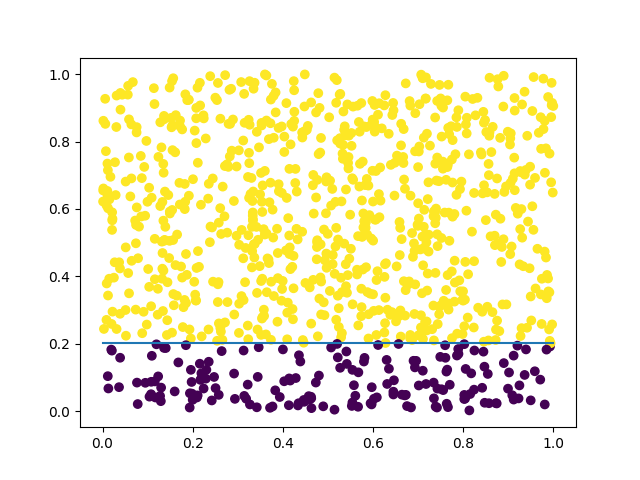
\includegraphics[width=0.8\textwidth]{../plots/d1_tree_viz.png}
    \caption{Scatter of D1.txt data with visualizations of decision tree boundaries.}
    \label{fig:d1_tree_viz}
  \end{figure}

  \begin{figure}[!h]
    \centering
    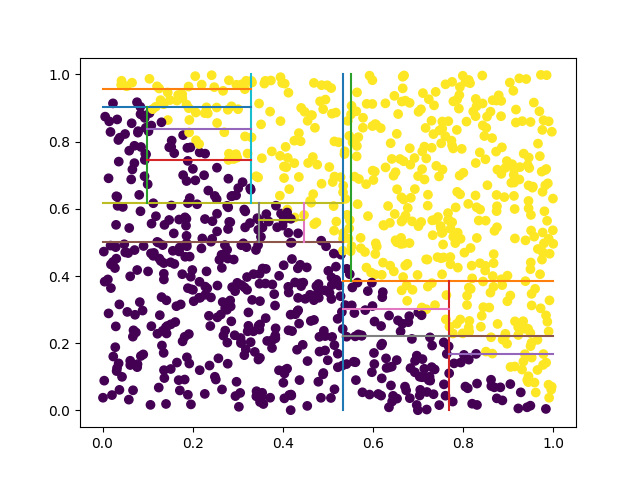
\includegraphics[width=0.8\textwidth]{../plots/d2_tree_viz.png}
    \caption{Scatter of D2.txt data with visualizations of decision tree boundaries.}
    \label{fig:d2_tree_viz}
  \end{figure}

  The size of the decision trees produced by the D1.txt and D2.txt data differ because of the hypothesis space of our decision tree algorithm.
  Our algorithm only considers splits on one dimension, which limits the hypothesis space of our algorithm.
  From figure \ref{fig:d2_tree_viz}, we can clearly see that the data is split on the line $x2 + x1 = 1$.
  If we were to have decision boundaries that considered linear combinations of features, I would anticipate the size of the trees would be the same.
\end{soln}

\item (Learning curve)  [20 pts] We provide a data set Dbig.txt with 10000 labeled items.  Caution: Dbig.txt is sorted.
  \begin{itemize}
  
  \item You will randomly split Dbig.txt into a candidate training set of 8192 items and a test set (the rest).  Do this by generating a random permutation, and split at 8192.
  
  \item Generate a sequence of five nested training sets $D_{32} \subset D_{128} \subset D_{512} \subset D_{2048} \subset D_{8192}$ from the candidate training set.  The subscript $n$ in $D_n$ denotes training set size.  The easiest way is to take the first $n$ items from the (same) permutation above.  This sequence simulates the real world situation where you obtain more and more training data.
  
  \item For each $D_n$ above, train a decision tree.  Measure its test set error $err_n$.  Show three things in your answer: (1) List $n$, number of nodes in that tree, $err_n$. (2) Plot $n$ vs. $err_n$.  This is known as a learning curve (a single plot). (3) Visualize your decision trees' decision boundary (five plots). \\
  \end{itemize}
  
\end{enumerate}

\begin{soln}
  \begin{center}
    \begin{tabular}{|c|c|c|}
      \hline
      $n$ & Tree Nodes & $err_n$ \\
      \hline
      32  &  0  &  0.3944  \\
      128  &  2  &  0.3944  \\
      512  &  7  &  0.2334  \\
      2048  &  6  &  0.172  \\
      8192  &  13  &  0.1781  \\
      \hline
    \end{tabular}
    \end{center}

    \begin{figure}[H]
      \centering
      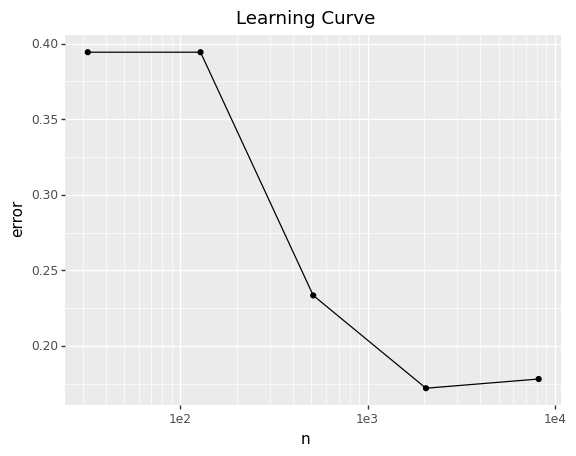
\includegraphics[width=0.8\textwidth]{../plots/error_curve.png}
      \caption{Learning curve}
      \label{fig:error_curve} 
    \end{figure}

    \begin{figure}[H]
      \centering
      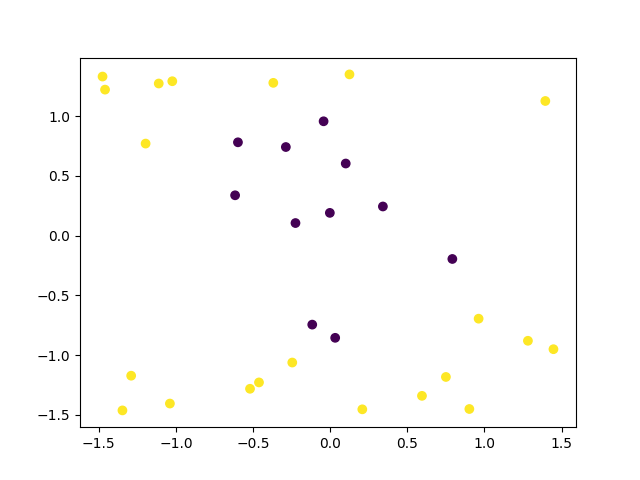
\includegraphics[width=0.8\textwidth]{../plots/dbig_32.png}
      \caption{Tree visualization for $n = 32$}
      \label{fig:dbig_32}
    \end{figure}
    
    \begin{figure}[H]
      \centering
      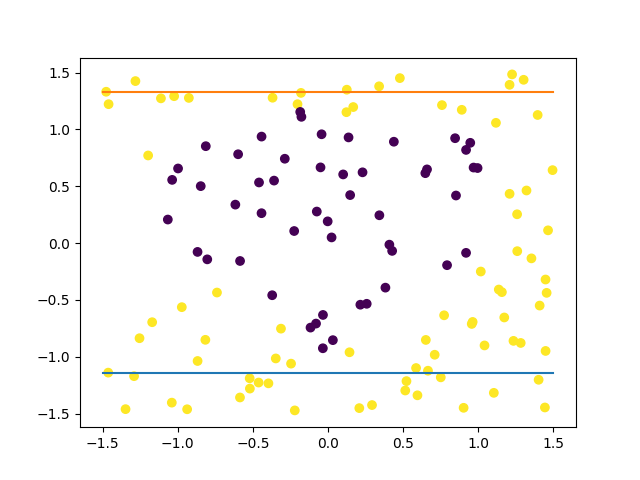
\includegraphics[width=0.8\textwidth]{../plots/dbig_128.png}
      \caption{Tree visualization for $n = 128$}
      \label{fig:dbig_128}
    \end{figure}

    \begin{figure}[H]
      \centering
      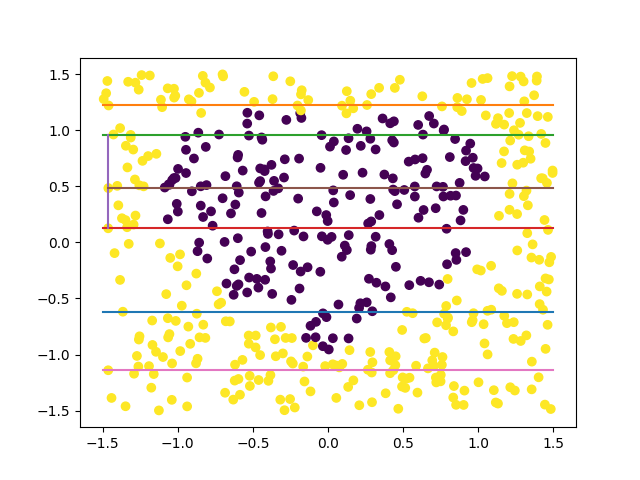
\includegraphics[width=0.8\textwidth]{../plots/dbig_512.png}
      \caption{Tree visualization for $n = 512$}
      \label{fig:dbig_512}
    \end{figure}

    \begin{figure}[H]
      \centering
      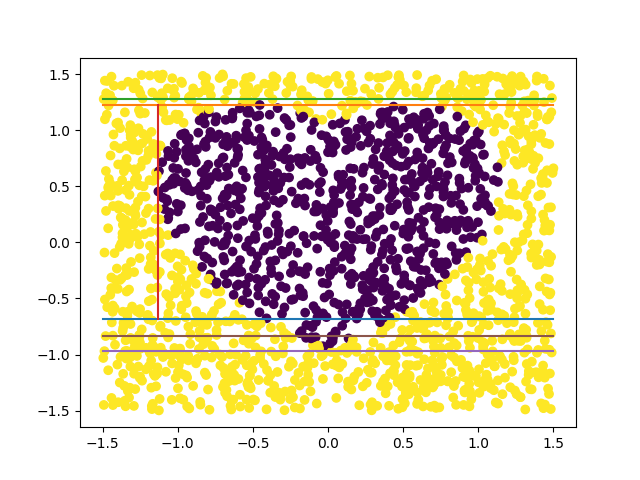
\includegraphics[width=0.8\textwidth]{../plots/dbig_2048.png}
      \caption{Tree visualization for $n = 2048$}
      \label{fig:dbig_2048}
    \end{figure}

    \begin{figure}[H]
      \centering
      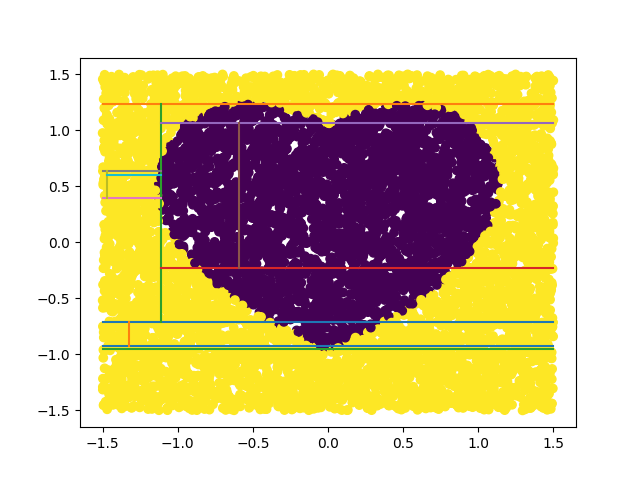
\includegraphics[width=0.8\textwidth]{../plots/dbig_8192.png}
      \caption{Tree visualization for $n = 8192$}
      \label{fig:dbig_8192}
    \end{figure}
  \end{soln} 

\section{sklearn [10 pts]}
Learn to use sklearn (\url{https://scikit-learn.org/stable/}).
Use sklearn.tree.DecisionTreeClassifier to produce trees for datasets $D_{32}, D_{128}, D_{512}, D_{2048}, D_{8192}$.  Show two things in your answer: (1) List $n$, number of nodes in that tree, $err_n$. (2) Plot $n$ vs. $err_n$.

\begin{soln}
  \begin{center}
    \begin{tabular}{|c|c|c|}
      \hline
      $n$ & Tree Nodes & $err_n$ \\
      \hline
      32  &  9  &  0.1383  \\
      128  &  23  &  0.073  \\
      512  &  41  &  0.0586  \\
      2048  &  111  &  0.0243  \\
      8192  &  243  &  0.0149  \\
      \hline
    \end{tabular}
  \end{center}

  \begin{figure}[H]
    \centering
    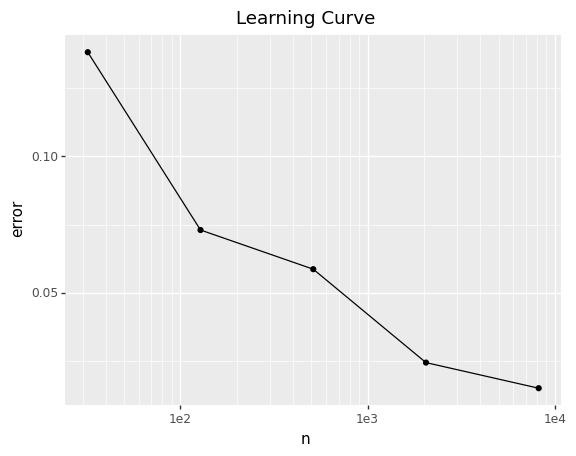
\includegraphics[width=0.8\textwidth]{../plots/sklearn_error_curve.png}
    \caption{Learning curve}
    \label{fig:sklearn_error_curve} 
  \end{figure}
\end{soln}

\section{Lagrange Interpolation [10 pts]}
Fix some interval $[a, b]$ and sample $n = 100$ points $x$ from this interval uniformly. Use these to build a training set consisting of $n$ pairs $(x, y)$ by setting function $y = sin(x)$. \\

Build a model $f$ by using Lagrange interpolation, check more details in \url{https://en.wikipedia.org/wiki/Lagrange_polynomial} and \url{https://docs.scipy.org/doc/scipy/reference/generated/scipy.interpolate.lagrange.html}. \\

Generate a test set using the same distribution as your test set. Compute and report the resulting model’s train and test error. What do you observe?
Repeat the experiment with zero-mean Gaussian noise $\epsilon$ added to $x$. Vary the standard deviation for $\epsilon$ and report your findings.

\begin{soln}

  For all experiments I samples from the interval $[-3, 3]$ and use MSE as my measure of error.

  \begin{center}
    \begin{tabular}{|c|c|c|}
      \hline
      $n$ & Train Error & Test Error \\
      \hline
      10  &  4.3835e-22  &  6.9074e-07  \\
      20  &  1.4873e-07  &  8.7370e-07  \\
      50  &  3.0097e+30  &  6.3737e+29  \\
      \hline
    \end{tabular}
  \end{center}

  The table above shows the results from the first experiment I ran using Lagrange interpolation.
  The documentation from scipy.org says that the algorithm is not stable for $n > 20$ so I tried the experiment with several different $n$.
  We find that when $n=10$, the error on the training data is several orders of magnitude smaller than the error on the testing data.
  When $n=20$, the training error is still smaller than the testing error but by a significantly smaller margin.
  Finally, when $n=50$, the training error is actually bigger than the test error.

  \begin{center}
    \begin{tabular}{|c|c|c|c|}
      \hline
      $n$ & $\sigma$ & Train Error & Test Error \\
      \hline
      15  &  .5 & 1782.7832  &  23238.8291  \\
      15  &  1 & 10025899609.8926  &  1879476606.1438 \\
      15  &  2 & 111.9039  &  340.1059  \\
      15  &  5 & 12447544.4681  &  12549414.3277  \\
      \hline
    \end{tabular}
  \end{center}

  The table above shows the results for the second experiment I ran using Lagrange interpolation.
  In this experiment, I trained the Lagrange polynomial with some noise $\epsilon$ added to the $x$-values, where $\epsilon \sim \mathbf{N}(0, \sigma)$.
  I fixed the $n=15$ for all trials to isolate the effect of $\sigma$ on the error.
  The results on interesting, at first as $\sigma$ increases from .5 to 1 the error for both training and testing data increases.
  But, from 1 to 2 the error decreases for both the training and testing data.
  When sigma changes from 2 to 5, $\sigma$ increases again.
  In every trial, the train error was less than the testing error.
  What I gather from these results is that there is some level of random noise you can add to the model to prevent overfitting the data.
  However, choosing $\sigma$ could be difficult.
\end{soln}



\bibliographystyle{apalike}
\end{document}
